\documentclass{article}
\usepackage[utf8]{inputenc}
\usepackage{mathtools}
\usepackage{amssymb}
\usepackage{graphicx}
\usepackage{listings}
\usepackage{float}
\usepackage{gensymb}
\usepackage{amsthm}
\usepackage{longtable}
\usepackage{adjustbox}
\usepackage{physics}
\usepackage{dsfont}

\theoremstyle{definition}
\newtheorem{definition}{Definition}
\newtheorem{example}{Example}
\newtheorem{theorem}{Theorem}
\newtheorem{claim}{Claim}

\title{Quantum Field Theory}
\author{quinten tupker}
\date{October 7 2020 - \today}

\begin{document}

\maketitle

\section*{Introduction}

These notes are based on the course lectured by Professor Nicholas Dorey in Michaelmas 2020.
This was lectured online due to measures taken to counter the spread of Covid-19
in the UK. These are not necessarily an accurate representation of what was
lectures, and represent solely my personal notes on the content of the course,
combinged with probably, very very many personal notes and digressions... Of
course, any corrections/comments would be appreciated.

But, let's actually introduce the content of this course. What is quantum field
theory? Quantum field theory (QFT) essentially succeeds in merging special
relativity
and quantum mechanics. Why is this so difficult? The first relativistic theory
was electromagnetism, and the biggest idea that was introduced, and what truly
set it apart from older theories was the idea of fields. In Newtonian theory, and much of what
followed, the protagonist of the theory was a particle, or if not a particle, at
least a body of some kind. Field theory changed. Now, there was a new
protoganist: the field. What difference does that make, architectually? Firstly,
the field theory is often simpler. But more importantly, the biggest structural
difference is that field theory excels in describing ``delayed interactions.''
When the particle is the progagonist, it is very difficult describe theories
where forces are not instantaneous. Field theory avoids this. All interactions
are made through the field, through which they propogate through space. Now,
delayed responses become natural. In electromagnetism, the simplest expression
thereof is electromagnetic waves: light. 

What does this have to do with relativity? Well, as soon as high speeds become
relevant, forces can no longer be considered instantaneous. As such, it is
difficult to keep using particles as the protoganist of these theories.
Consequently, the natural step is to make, instead of particles, fields the
protoganist of this new quantum theory we are developing.

That is the goal of QFT. There is one important consequence though, once
particles are no longer the protagonists of the theory. That is that particle
number no longer has to be conserved. In the most elegant fashion, by removing
the supremacy of the ``particle'' in our theory, and replacing it with the more
powerful notion of the field, particles merely become phenomenon to be observed,
and tools of analysis. In this context, it is only natural that particle number
is no longer conserved. Whereas before, the wavefunction was often associated
with a wave-particle like object, now the wavefunction (which is a field)
describes a multiparticle state. Well, really it describes the field, and the
multiparticle state is something that can be deduced from it. Somehow, although
this is just the beginning of the course, I feel that that's not that important
anymore. It is deeply intriguing though, how the imposition of boundary
conditions somehow forces a degree of discreteness onto this theory...

Well then, the overall architecture is more or less the same as standard quantum
theory. It is probabilistic, and we assume a degree of symmetry under
boosts, and rotations (isotropy and translation invariance). The fundamental
approach to making predictions still boils down to the same calculation:
evaluating

$$ A_{i \to f} = \bra{f} e^{i H T} \ket{i} $$

for probability amplitude $A$, initial state $i$, final state $f$, Hamiltonian
(time translation generator) $H$, and time interval $T$.

There are two caveates with most of these field theories, though. Firstly, they
have not been mathematically formalised, so often there are areas that are
somewhat ambiguous. Secondly, contributing to this ambiguity, many of the sums
are divergent, so the meaning of some calculations can really be somewhat
ambiguous... How curious! I'd like to think about this a bit more...

\section{Preliminaries}

Anyways, getting down to business. We'll be mostly using natural units during
this course. That means that $c = \hbar = 1$, and these can be added back into
the calculation using dimensional analysis. The effect of this, is that the only
unit used throughout all calculations is really a unit of mass-energy. As such,
all quantities scale by a power of the unit of energy. 

\begin{definition}[dimension of $X$]
  Denoted $[X]$, this is $\delta$, such that for unit of mass-energy $M$, $X$
  scales as $M^\delta$. $\delta$ may also be called the scaling or the
  engineering dimension of $X$.
\end{definition}

Also, for special relativity we use the convention that we are working on
Minkowsky space-time $\mathbb{R}^{3, 1}$, with metric tensor

$$ \eta_{\mu \nu} = \text{diag}(1, -1, -1, -1). $$

\section{Classical Field Theory}

Fortunately for me, we are starting with a description of classical field
theory, and we are starting, very simply, with scalar fields.

\begin{definition}[Scalar Field]
  $\phi(t, \underline{x}) = \phi(x) : \mathbb{R}^{3, 1} \to \mathbf{R}$ is a sclar field
  if it is Lorentz invariant, meaning that it follows the transformation rule
  $$ \phi(x) \to \phi(\Lambda^{-1}(x)) $$
  Here the domain is called the spacetime, and the codomain is called the
  \textbf{field space}. These may, and will be replaced with other spaces.
\end{definition}

Changing the spacetime here corresponds to implementing gravity in some way or
another, by changing the manifold we are working on. The field space corresponds
to the complexity of what is being descibed. Since we will be describing
multi-particle states with our wavefunction, this will become significantly more
complex. And, I intentionally left the description of what it means to be
Lorentz invariant a bit vague, since, well, in our case, it just means being
invariant under the Lorentz transformations, which is the group of
linear transformations that preserves the Minkowsky metric (ie. the set of
matrices such that $\Lambda \eta \Lambda^T = \eta$). But really, while linearity
makes a lot of sense in the context of linear Minkowsky space, I doubt (though I
have no familiarity with this area) this remains the case when we are on an
arbitrary manifold, which happens when we consider general relativity. As such,
I prefer to think of $\Lambda$ as any arbitrary invertible map on the manifold,
corresponding to the symmetries we impose. 

The difficulties that arise in comibing quantum theory with general relativity
are also quite clear. It does seem tremendously difficult. If we do not simply
assuming that general relativity simply bends space, which I will assume is not
entirely the case, or else I feel a theory reconciling the two would have
already been developed long ago, in spite of the tremendous difficulty of the
calculations involved, and it also does not seem to make much sense of Hawking
radiation, since in general relativity, the space at the centre of a black hole
truly is cut off... Nevertheless, from what I've heard, if you want to turn
gravity into a quantised force with mediator particle, then somehow the
protagonist of that theory would be not only be a field, but somehow span the
space of possible manifolds as well. Purely intuitively, I would imagine that we
would be getting fields of the form $\phi : \mathcal{D} \to V$ where
$\mathcal{D}$ is an object that stitches many manifolds together. Brrr... I have
not thought too deeply about this, but that does seem like a truly terrifying
object indeed! Or perhaps not quite. Hm, it might be worth thinking a bit more
about this...

Anyways, I also wanted to remark that having fields transform as
$\phi(\Lambda^{-1}x)$ is more or less an arbitrary definition that is called the
``active'' definition of field transformations. Oh well, you can assign some
intuition to it, but it is more or less convention to use the inverse of the
matrix instead of the matrix itself.

Extending our notion of fields to vector fields, first note that notation wise,
we use $\partial_\mu \phi = \frac{\partial \phi}{\partial x^\mu}$, and we define

\begin{definition}[$\phi^\mu$ transforms as a vector field]
  if
  $$ \phi \to \Lambda^\mu_\nu \phi^\nu (\lambda^{-1} x) $$
\end{definition}

This is just the transformation rule for rank 1 tensors, so is nothing
particularly remarkable. The only remarkable part is that, as a result
$\partial^\mu \phi$ transformas as vector, and so the following becomes a rank 0
tensor (ie, a scalar field) $\partial^\mu \phi \partial_\mu \phi$.

Well, that ends [lecture 1], for those of you interested. 

\subsection{The Lagrangian}

We will review some of the tools from classical mechanics that we are using. The
first is the Lagrangian. There are three advantages to using the lagrangian
here:

\begin{itemize}
\item they are independent of coordinates
\item the symmetries of the system can be easily expressed
\item the path integral formulation follows immediately
\end{itemize}

although the Lagrangian is used much more heavily in the Advanced Quantum Field
Theory course than the current course. Anyways, we review the Lagrangian, except
that now we implement it on fields, so $L = L(\phi, \partial_\mu \phi)$ for
(scalar) fields $\phi$, and we make three requirements of our action/Lagrangian

\begin{itemize}
\item The action $S$ is Lorentz invariant
\item we require locality (see below)
\item we have at most a second order time derivative
\end{itemize}

Locality essentially means that $L = \int dx^3 \, \mathcal{L}(\phi(x),
\partial_\mu \phi(x))$, so the Lagrangian has an associated local Lagrangian
density $\mathcal{L}$. From hereon, this $\mathcal{L}$ will usually be referred
to as the Lagrangian instead. We note that the action (over an infinite time
scale) may now be expressed as

$$ S = \int dx^4 \mathcal{L}(\phi, \partial_\mu \phi) $$

Now, Lorentz invariance essentially means that the Lagrangian density is a
scalar field (a tensor really), meaning that it transforms as $\mathcal{L}(x)
\mapsto \mathcal{L}(\Lambda^{-1} x)$. This corresponds to the action being
Lorentz invariant since the Jacobian of a Lorentz transformation (the
determinant) is 1, so the relevant change of variables, the action does not
change.

Finally, using no more than a second order time derivative in the context of
relativity means using no more than a second order derivative of any kind, and
since we also are rank-0 tensors, we in fact, cannot have first order
derivatives either. Consequently, we can write the general form of the
Lagrangian as 

$$ \mathcal{L} = \frac{1}{2} F(\phi) \partial_\mu \phi \partial^\mu \phi - V(\phi) $$

(note that $\phi \partial_\mu \partial^\mu \phi$ is related to the above by
integration by parts so can be safely ignored). Also, in practice in quantum
theory we may neglect $F(\phi)$ leaving us with quite a simple general form.

To make all this work, we apply the principle of least action, which gives us
the Euler Lagrange equation

$$ \partial_\mu \partial_{\partial_mu \phi} \mathcal{L} = \partial_\phi
\mathcal{L} $$

An important special case to consider is the case when the potential is
quadratic, so $V(\phi) = \frac{1}{2} M^2 \phi^2$, which means the Euler-Lagrange
case is linear, leaving us with the so-called \textbf{Klein-Gordon Equation}

$$ \partial_\mu \partial^\mu \phi + M^2 \phi = 0 $$

As one might expect, since in Minkowski spacetime $\partial_\mu \partial^\mu =
\partial_t^2 - \nabla^2$ we get wavelike solutions

$$ \phi \sim e^{ix \cdot p} $$

where $x \cdot p = \omega t - \vec{k} \cdot \vec{x}$, and the dispersion
relation requires $\omega_k = \sqrt{k^2 + M^2}$.

On a philosophical note, I was wondering what difference using the principle of
least action makes compared to just Newton's equations (on a philosophical level
- it is obviously more practical), and as such I was wondering to what extent
the Lagrangian formulation in a sense is just a tensor formulation of Newton's
equations? 

I also was wondering what locality means. When discussing life, I have remarked
that really as long as one is not starving, etc., reality is little more than a
medium for communication between people. This is certainly the case for
particles, and objects, which do not have to worry about starvation, etc. But
then I wonder, do particles really not need to worry about starvation? Many
particles decay after all, although I doubt that has to do with a kind of
starvation of any kind... [End of lecture 2]

\subsection{Maxwell's Theory}

Maxwell's theory uses a 4-vector potential $A^\mu = (\phi, \vec{A})$. This being
a rank 1 tensor means it transforms as

$$ A^\mu(x) \mapsto \Lambda^\mu_\nu A^\nu(\Lambda^{-1} x) $$

In electromagnetism, the \textbf{field strenght tensor} is given by

$$ F^{\mu \nu} = \partial^\mu A^\nu - \partial^\nu A^\mu $$

and as a tensor, it transforms as appropriate. But it satisfies a further
condition that it is invariant under Gauge transformations $A^\mu \mapsto A^\mu
+ \partial^\mu \lambda$. This leads to the \textbf{Bianchi identity}

$$ \partial_\lambda F_{\mu \nu} + \partial_\mu F_{\nu \lambda} + \partial_\nu
F_{\lambda \mu} = 0 $$

which captures 2 out of Maxwell's 4 equations. The other two arise from the
principle of least action applied to the \textbf{Maxwell Lagrangian}

$$ \mathcal{L} = -\frac{1}{4} F_{\mu \nu} F^{\mu \nu} $$

We should note that there really are not that many options of Lagrangians here
once one introduces the standard assumptions in addition to assuming it must be
expressed in terms of physical quantities (the only candidate is the field
strength vector used above)... Writing

$$ \mathcal{L} = -\frac{1}{2} \partial_\mu A_\nu \partial^\mu A^\nu +
\frac{1}{2} (\partial_\mu A^\mu)^2 \eta^{\mu \nu} $$

gives us (after Euler-Lagrange)

$$ \partial_\mu F^{\mu \nu} = 0 $$

which provides us with the rest of the Maxwell equations.

\subsection{Symmetries in QFT}

Symmetries (see the Symmetries, Fields, and Particles (SFP) course) are variations of
fields that leave the action invariant. Symmetries have several effects in
physics. Firstly, by Noether's theorem, they lead to conservation laws.
Secondly, they restrict the form of the Lagrangian. In particular, Gauge
symmetry is very powerful due to strong restrictions it puts on the form of the
Lagrangian. 

Common symmetries include (See SFP) translation invariance and Lorentrz
transformation invariance. Another symmetry occurs when either $m = 0, V = 0$ or
the action is propoertional to the field. In this case we get an additional
``scale invariance'' where $x^\mu \mapsto \lambda x^\mu$ and $\phi \mapsto
\lambda^{-\Delta} \phi(\lambda^{-1}x)$ for engineering constant $\Delta$.

Internal symmetries like charge, flavour or colour conservation also occur,
further restricting the theory. These are not related to the space, and are
somehow better expressed by the quantity they conserve. Another small curious
symmetry is the following:

\begin{example}
For complex scalar fields with $\mathcal{L} = \partial_\mu \psi^* \partial^\mu
\psi - V(|\psi|^2)$ the following is also a symmetry: $\psi \mapsto e^{i \alpha}
\psi$ for real $\alpha$. The lecturer does not go into any more detail about
this.
\end{example}

Finally, we note that for continuous symmetries, which form Lie groups, we can
take the set of elements of the group ``near'' the identity, $g = e^{\alpha X}$
where $X$ sits in the Lie algebra of $G$. Working to 1st order we now may write

$$ g \cdot \psi \mapsto \psi + \delta \psi = \psi + \alpha X \psi $$

to first order. [End of lecture 3]

Just as a remark on terminology, a Lorentz transformation is a linear
transformation preserving the Minkowski metric. On the other hand, a
\textbf{proper Lorentz transformation} is a Lorentz transformation with
determinant 1 (which ensures causality). 
Our goal now is to work towards Noether's theorem. Noether's theorem states that \begin{theorem}[Noether's Theorem] For every continuous symmetry, there exists a conserved current, given by
  $$ j^\mu = \partial_{\partial_\mu \phi} \mathcal{L} \delta \phi -
  F^\mu(\phi(x)) $$
  where $\delta \phi$ is the variation in $\phi$ and $\delta \mathcal{\lambda} =
  F^\mu$.
  Conservation here means that $\partial_\mu j^\mu = 0$.
\end{theorem}

The conserved quantity associated with the conserved current then can be shown
to be $Q = \int dx^3 j^0$ since

\begin{align*}
  \frac{d}{dt} Q
  &= \int dx^3 \partial_t j^0 \\
  &= - \int dx^3 \nabla \cdot J \\
  &= \int_S dS \cdot J \\
  &= 0
\end{align*}

A good example is $j^\mu = (\rho, J)$ for charge density and current in
electromagnetism. Anyways, here is our ``proof'' of Noether's theorem:

\begin{proof}
  Using the Euler-Lagrange equation applied to the field $\phi$ we see that
  \begin{align*}
    \delta \mathcal{L}
    &= \partial_\phi \mathcal{L} \delta \phi + \partial_{\partial_\mu \phi} \mathcal{L} \delta \partial_\mu \phi \\
    &= (\partial_\phi \mathcal{L} - \partial_\mu (\partial_{\partial_\mu \phi} \mathcal{L})) \delta \phi + \partial_\mu (\partial_{\partial_\mu \phi} \mathcal{L} \delta \phi) \\
    &= \partial_\mu (\partial_{\partial_\mu \phi} \mathcal{L} \delta \phi)
  \end{align*}

  Then using our definition of $j^\mu$ as above we see that $\partial_\mu j^\mu
  = 0$.
\end{proof}

Here it is assumed that $\delta \mathcal{L} = \partial_\mu F^\mu$ which means we
can apply Stokes' theorem and integrate on the surface only. When we do so,
$F^\mu$ becomes that surface term we integrate with. But Euler-Lagrange also
means that our expression above, for the first term in the conserved current, is
also a surface term (often determined by the boundary conditions) for $\delta
\mathcal{L}$. So what exactly is the difference? Is it that the first term
depends on the variation whereas the second does not?

[End of lecture 4 - this bit needs rewriting]

[Start of Noether's theorem rewrite]

Alright, so now to the main topic of this lecture: Noether's theorem. Noether's
theorem states that for every continuous symmetry we get a conserved current
(and quantity), which she gives an equation for. Now how do we get that?

Firstly, we observe that for a Lorentz transformation

$$ \Lambda \approx I + s\Omega $$

where $\Omega$ is antisymmetric (to ensure we preserve the Minkowski metric). If
that the case, we see that if we tree $\mathcal{L}$ as a scalar field
$\mathcal{L}(x)$ instead of a function of the field, then

$$ \delta \mathcal{L} = - s\Omega^\mu_\nu x^\nu \partial_\mu(\mathcal{L}(x)) =
-s\Omega^\mu_\nu \partial_\mu (x^\mu \mathcal{L}(x)). $$

This last equality only holds because $\Omega$ is asymmetric (so its diagonal is
all zeros). But importantly, we see that $\delta \mathcal{L}$ can be written as
a total derivative when $x$ is varied.

Now, we vary the same $\mathcal{L}$ but instead of varying with respect to $x$,
we vary with respect to the field $\phi$. Doing so, and assuming Euler-Lagrange
we find that:

\begin{align*}
  \delta \mathcal{L}
  &= \partial_\phi \mathcal{L} \delta \phi + \partial_{\partial_\mu \phi} \mathcal{L} \delta \partial_\mu \phi \\
  &= (\partial_\phi \mathcal{L} - \partial_\mu (\partial_{\partial_\mu \phi} \mathcal{L})) \delta \phi + \partial_\mu (\partial_{\partial_\mu \phi} \mathcal{L} \delta \phi) \\
  &= \partial_\mu (\partial_{\partial_\mu \phi} \mathcal{L} \delta \phi)
\end{align*}

Remarkably, we find once again that we may write $\delta \mathcal{L}$ as a total
derivative. Let us now denote these variations as $\delta_x \mathcal{L}$ for the
first, and $\delta_\phi \mathcal{L}$ for the second. Now, since we have a
symmetry, we know that the action is unchanged when we apply a Lorentz
transformation. In particular, we know that the ``partial variation'' of
$\mathcal{L}$ with respect to $x$ alone, but ignoring $\phi$ should be
``constant.'' What do we mean by constant? The partial derivative with respect
to space is a 4-vector, so really we mean that the Minkowski metric is
unchanged. In other words, to first order the quantity

$$ v_M \cdot \partial_x \delta \mathcal{L} = 0 $$

where we use $\partial_x \delta$ to denote this ``pure'' partial derivative and

$$
v_M =
\begin{pmatrix}
  -1 \\
  1 \\
  1 \\
  1
\end{pmatrix}
$$

is the ``Minkowski vector'' (the first order derivative of the Minkowski metric
in a sense). This would mean that the Minkowski metric is unchanged under a pure
variation of spacetime. So how do we write this pure variation of space time?
We notice that $\delta \partial_x \mathcal{L} = \delta_x \mathcal{L} -
\delta_\phi \mathcal{L}$ since in a sense $\delta_x \mathcal{L}$ is the total
derivative of $\mathcal{L}$ with respect to $x$, and $\delta_\phi \mathcal{L}$
is the total derivative of $\mathcal{L}$ with respect to $\phi$, and so, by the
chain rule, what is left over is the partial variation with respect to $x$.

This is exactly what Noether's theorem refers to. Noether's theorem defines the
\textbf{conserved current} to be

$$ j^\mu = \partial_{\partial_\mu \phi} \mathcal{L} \delta \phi - F^\mu $$

where $\delta_x \mathcal{L} = \partial_\mu F^\mu$, and $\delta_\phi \mathcal{L}
= \partial_\mu (\partial_{\partial_\mu \phi} \mathcal{L} \delta \phi) $, and so
we see that our partial variation of $\mathcal{L}$ with respect to only $x$ is

$$ \delta \partial_x \mathcal{L} = -\frac{\partial}{\partial x_\mu} j^\mu $$

(no summation convention - this is a vector here), and importantly

$$ \partial_\mu j^\mu = v_M \cdot \delta \partial_x \mathcal{L} = 0 $$

as required since $\partial_\mu j^\mu = \delta \mathcal{L} - \delta \mathcal{L}
= 0$.

That is Noether's theorem. I do not fully understand it, and to me it seems
weird that the ``generators'' of these variations (the terms like $F^\mu$ inside
the derivative) are not the same. But anyhow, Noether's theorem states that
$j^\mu$ is conserved, so $\partial_\mu j^\mu = 0$ (which means the Minkowski
metric stays the same in the way we described). Aside from that we will remark
that we assume in general that for any symmetry $\partial_x \mathcal{L} =
\partial_\mu F^\mu$ for some $F^\mu$,

Now where does a conserved quantity arise from. Here we note that if $Q = \int
dx^3 j^0$ then it satisfies

\begin{align*}
  \frac{d}{dt} Q
  &= \int dx^3 \partial_t j^0 \\
  &= - \int dx^3 \nabla \cdot J \\
  &= \int_S dS \cdot J \\
  &= 0
\end{align*}

and os is conserved. One can check that in the case of electromagnetism, $Q$
corresponds precisely to electromagnetic charge.

[End of Noether's theorem rewrite]

Today we will look at certain examples of Noether's theorem. In particular, we
will define the energy-momentum constant as the Noether current arising from
translation invariance. Under the symmetry $x^\mu \mapsto x^\mu + \epsilon^\mu$,
we get $\phi \mapsto \phi(x - \epsilon) \approx \phi(x) - \epsilon^\mu
\partial_\mu \phi + \dots$. We also get $\delta \mathcal{L} = -\epsilon^\mu
\partial_\mu \mathcal{L}$. Consequently we get energy-momentum tensor

$$ T^\mu_\nu = j^\mu_\nu = \partial_{\partial_\mu \phi} \mathcal{L} \partial_\nu
\phi - \delta^\mu_\nu \mathcal{L} $$

As Noether current, this is conserved, meaning $\partial_\mu T^\mu_\nu = 0$. We
consequently get conserved quantities:

$$ E = \int d^3x T^{00} $$
$$ p^i = \int d^3xT^{0i} $$

or equivalently, the 4-momentum is conserved:

$$ p^\nu = \int d^3x T^{0\nu}. $$

[Lecturer computes example in Klein-Gordon case.] In many cases, such as the
Klein-Gordon case we find the energy-momentum tensor to be symmetric, but this
need not be the case in general. However, just as the Lagrangian gives rise to
the same physics if we add a total derivative, one can show that the
energy-momentum tensor has a similar symmetry, and if a particular choice of
total derivative is made, we find that we can always make $T^{\mu \nu}$
symmetric.

More specifically, we find that if we use the formula from general relativity
for the energy-momentum tensor:

$$ T_{\mu\nu}(x) = \frac{-2}{\sqrt{-g}} \partial_{g^{\mu\nu}} (\sqrt{-g}
\tilde{\mathcal{L}}) $$

for $g = \text{det}(g_{\mu \nu})$ then we always get a symmetric result. By
using the Minkowski metric we can recover our original result.

\section{Canonical Quantisation}

In the Advanced Quantum Field Theory course in Lent, we will use the Lagrangian
directly to formulate the path integral version of quantum mechanics. Here,
however, we will stick to the Hamiltonian approach. For that we do a small
review of Hamiltonian mechanics by starting with the Lagrangian

$$ L(q, \dot{q}) = \frac{1}{2}\dot{q}^2 - V(q) $$

We then define the \textbf{momentum conjugate to $q$} to be $p =
\partial_{\dot{q}} L$. Performing the Legendre transform we then can define the
\textbf{Hamiltonian} to be

$$ H = p\dot{q} - \mathcal{L} = \frac{1}{2}p^2 + V(q) = H(p, q) $$

since $H$ is really seen as a functino of $p$ and $q$. It is also clear that
Hamiltonian can be seen as the total energy of a point in state space $(p, q)$.

Now, we generalise our system to $N$ particles as

$$ H = \sum_{i=1}^N p_i q_i - \mathcal{L} $$

and introduce the \textbf{Poisson
  bracket} (which is related to the commutator) as 

$$ \{F, G\} = \sum_{i = 1}^N \partial_{q_i} F \partial_{p_i} G - \partial_{p_i}
F \partial_{q_i} G $$

for functions $F, G$ of $p, q$. We can then get the following important result:
the Hamiltonian is the generator of time evolution, meaning that $\forall F(p,
q)$ we find

$$ \dot{F} = \{H, F\}. $$

An important special case of this is that we can write the principle of least
action by applying the time evolution property to $p$ and $q$ asking

\begin{align*}
  \dot{q}_i &= \{H, q_i\} = \partial_{p_i} H \\
  \dot{p}_i &= -\partial_{q_i} H
\end{align*}

and for any conserved $Q$, we get $\{H, Q\} = 0$. Finally, we note that these
also satisfy the property that

$$ \{q_i, p_j\} = \delta_{ij}$$

[End of lecture 5]

How do translate this Hamiltonian to field theory? Firstly we define the
\textbf{momentum conjugate to the field} as

$$ \pi = \partial_{\partial_{\dot{\phi}}} \mathcal{L} $$
and we apply the Legendre transform to get the \textbf{Hamiltonian density}

$$ \mathcal{H} = \pi \dot{\phi} - \mathcal{L} = \mathcal{H}(\phi, \pi) $$

and, as expected the normal Hamiltonian can then be calculated as

$$ H = \int d^3x \mathcal{H}. $$

As a check, and example, if we use $\mathcal{L} = \frac{1}{2}\partial_\mu \phi
\partial^\mu \phi - V(\phi)$ (a ``suitably'' general Lagrangian) we get

$$ \mathcal{H} = \frac{1}{2} \dot{\phi}^2 + \frac{1}{2} | \nabla \phi|^2 +
V(\phi) = T^{00} $$

the energy density, as one might hope.

\subsection{The Canonical Quantisation}

Now to actually quantise things we convert the Poisson bracket $\{\}$ to the
commutator $\frac{1}{i\hbar} []$, with overall quantities staying the same. That
means that for $\pi, \phi$ we get that

$$ [\pi_i, \pi_j] = [\phi_i, \phi_j] = 0$$

but that

$$ [ \pi_i, \phi_j] = i\hbar \delta(x - y), $$

as one might expect. The time evolution property of $H$ becomes 

$$ H \ket{\psi} = -i \hbar \partial_t \ket{\psi}. $$

In particular that means that for any conserved quantity (commutes with $H$), we
can simultaneously diagonalise these to get a simultaneous basis $H$ and the
conserved quantity. Also, note here that we later set $\hbar = 1$.

Anyways, using the standard Hamiltonian approach we then find that

$$ H = \int d^3x \frac{1}{2} \pi^2 + \frac{1}{2} |\nabla \phi|^2 + V(\phi) $$

In practice, this is very hard to calculate, so not very helpful (one would have
to diagonalise this function to find the energy eigenstates...). Instead we find
some other ways.

Finally, on interpretation, we note that the eigenvalues have become functions
$f : \mathbb{R}^3 \to \mathbb{R}$, which we assume span the Hilbert space as
usual. However, this has never been formalised mathematically, so it is a bit of
a grey area... [End of lecture 6]

In general, solving this Hamiltonian works out to be a functional differential
equation, which is predictably hard. Instead, we tend to work with special
cases. That is how we will proceed.

\subsection{Free Field Theory}

The simplest case is to assume everything is non-interacting, and that the
Lagrangian obeys the Klein-Gordon equation. That means we are left with

$$ \mathcal{L} = \frac{1}{2} \partial_\mu \phi \partial^\mu \phi -
\frac{m^2}{2}\phi^2 \implies \partial_\mu \partial^\mu \phi + m^2 \phi = 0 $$

We can solve this using a Fourier transform to get

$$ (\partial_t^2 + |p|^2 + m^2) \tilde(\phi) = 0 $$

which has solutions for $\omega_p = \sqrt{|p|^2 + m^2}$ of the form

$$ \tilde{\phi} = A_p e^{-i\omega_p t} + B_p e^{-i\omega_p t} $$

which form the modes of a Harmonic oscillator. In fact, calculating the action
we find

$$ S = \frac{1}{2} \int dt \int \frac{d^3p}{(2\pi)^2} \tilde{\phi}^*
(-\partial_t^2 - |p|^2 - m^2) \tilde{\phi} $$

which means really do get a infinite number of decoupled complex simple harmonic
oscillators. This is essential, since it is this simplicity locally that gives
us a chance at solving the problem at all!

\subsubsection{The Quantum Simple Harmonic Oscillator (review)}

Firstly, though, let's review the quantum simple harmonic oscillator (SHO) so
that we can use it for comparison. In this case

$$ L = \frac{1}{2} \dot{q}^2 - \frac{\omega^2}{2} q^2 \implies H = \frac{p^2}{2}
+ \frac{\omega^2}{2}q^2 $$

We can quantise this as usual for $p, q$, and then solve it using general
methods. The unique aspect of the SHO though is that we can use purely its
algebra to gain a solution by considering the raising and lowering/ladder
operators

$$ a = \sqrt{\frac{\omega}{2}} q + \frac{i}{\sqrt{2\omega}} p, a^\dagger =
\sqrt{\frac{\omega}{2}} q - \frac{i}{\sqrt{2\omega}} p $$

where we find $[a, a^\dagger] = \hbar$, which crucially means that

$$ H = \frac{1}{2}\omega(aa^\dagger + a^\dagger a) = \omega(a^\dagger a +
\frac{1}{2}\hbar) $$

where one can identify $N = a^\dagger a$ as the number operator. Even more
importantly we see that

$$ [H, a] = - \omega \hbar a, [H, a^\dagger] = \omega \hbar a^\hbar $$

The fact that the commutator is still proportional to $a, a^\dagger$ means that
when applied to an energy eigenstate, $a, a^\dagger$ either annihilate the
state, keep the same state, or create a new state. As such, we create the ladder
operators as usual, and we find a state $\ket{0}$ such that $a\ket{0} = 0$, but
we can define an inifite ladder of states $\ket{n} = (a^\dagger)^n \ket{0}$. The
energies of these states are given by $E_n = \hbar \omega(n + \frac{1}{2})$. 

\subsubsection{Back to Field Theory}

To generalise to field theory we might define our ladder operators as:

$$ \phi = \int \frac{d^3p}{(2\pi)^2} \frac{1}{\sqrt{2\omega_p}} \left( a_p
    e^{ip\cdot x} + a_p^\dagger e^{-ip \cdot x} \right) $$

$$ \pi = \int \frac{d^3p}{(2\pi)^2} (-i) \sqrt{\frac{\omega_p}{2}} \left( a_p
    e^{ip\cdot x} - a_p^\dagger e^{-ip \cdot x} \right) $$

If we gain the same commutation relations, from these definitions then we can
call ourselves satisfied that these definitions have the properties what we
want. As such, we wish to show that the following commutation relations

$$ [\phi(x), \phi(y)] = [\pi(x), \pi(y)] = 0, [\phi(x), \pi(y)] = i\delta(x -
y) $$

if and only ifoddpage

$$ [a_p, a_q] = [a_p^\dagger, a_q^dagger] = 0, [a_p. a_q^\dagger] = i\delta(x -
y) $$

Some algebra shows that indeed this is the case. 

Having shown that these definitions can make sense, we want to see if we can
calculate the energy eigenstates from here, as we do in the non-field theory
case. As such we calculate

$$ H = \frac{1}{2} \int d^3x (\pi^2 + |\nabla p|^2 + m^2 \phi^2) $$

by writing every term in terms of $a, a^\dagger$ and find that as expected

$$ H = \frac{1}{2} \int \frac{d^3p}{(2\pi)^3} \omega_p (a_p a_p^\dagger +
a_p^\dagger a_p) $$

[End of lecture 7] This calculation can be simplified by creating and eliminating delta functions
as soon as possible. So our first step here would be to calculate the ground
state energy, which in the context of field theory is called the ``vacuum'' (or
the energy of the vacuum). Doing so for $\ket{0}$ such that $a\ket{0} = 0$ we
find that

$$ H\ket{0} = \frac{1}{2} \int d^3 p \omega_p \delta(0) \ket{0} = \infty
\ket{0} $$

which points us to a general aspect of field theory: many things diverge. How do
we get around this? There are two types of divergence present here, which are
called \textbf{infrared divergence} (IR divergence) and \textbf{ultraviolet
  divergence} (UV divergence). IR divergence refers to divergence that occurs
due to the large distances (but possibly low energies) involved. Ultraviolet
divergence on the other hand occurs due to the high energies (but often short
distances) involved. The infrared divergence is relatively simple to solve: we
consider the energy density $\mathcal{E}$ instead of the total energy, which
makes sense since almost everything else we're working with is a density.
Formally this can be expressed as restricting the energy to a box of limited
size.

That solves the IR divergence, leaving us with

$$ \mathcal{E}_0 = \int \frac{d^3p}{(2\pi)^3} \frac{1}{2} \omega_p \sim \int
|p|^3 d|p| = \infty $$

(where exactly does this come from?), but we still have UV divergence. To
resolve this, we use a rather crude UV cutoff, which is an energy cutoff,
limiting our integrals to only energies lower than $\Lambda >> 1/m$ where $1/m$
is the only natural length scale available to us in this context. Calculating
$\mathcal{E}_0$ in this limit for $\Lambda$ gives us

$$ \mathcal{E}_0^\Lambda = \frac{1}{16 \pi^2} \Lambda^4 (1 + O(m^2 /
\Lambda^2)). $$

An alternative, and more intuitive approach would be to replace continuous
spacetime with a lattice. This does work, and gives a similar result in fact,
but is much harder to do. The equivalence between this relates to a somewhat
profound relationship between small distances and high energies, and in fact the
lattice spacing $a$ is inversely proportional to our energy cutoff in a certain
sense. 

Some interpretations can be offered for the situations we get here. One involves
the fact that we don't really know what happens at high energies, and so we
focus on where we know our field theory works (referred to as \textbf{effective
  field theory}). Another approach is that the method that we quantise our
theory is more or less arbitrary and so we could instead use a different
quantisation called the ``natural ordering'' which forces all terms involving
$a, a^\dagger$ to put $a$s in front, leaving $\mathcal{E}_0 = 0$. I don't know
how well this works in general.

Finally, another approach to this issue is simply not to care, since why should
inifinite energies really make a difference (closest to my attitude to the
situation). After all, we can only really measure energy differences in
experiment. That's not entirely true though, since once one starts to
incorporate gravity, one sees that through the energy-momentum tensor relativity
does introduce a certain absolute measure of energy... This relation remains a
relatively mysterious aspect of physics. [End of lecture 8]

To give some more detail on this relationship, we notice that the Einstein
equations $R_{\mu\nu} - \frac{1}{2} R g_{\mu \nu} = 8\pi G T_{\mu \nu}$ mean
that if we have constant vacuum energy $\bra{0} T_{\mu \nu} \ket{0} =
\mathcal{E}_0 g_{\mu \nu}$ essentially is equivalent to introducing a new
cosmological constant $\lambda$. This was significant,
especially since until around 20 years ago (~2000) the cosmological constant was
assumed to be 0. In truth though it  remains one of the greatest mysteries in
physics since $\lambda \sim \mathcal{E}_0 G \sim (10^{-3} \text{eV})^2$, while
if instead we assume that there is an energy cutoff around the Planck length
$\Lambda \sim M_L = \sqrt{\frac{\hbar c}{G}}$ then we find $\lambda \sim 10^{28}
\text{eV}$. So we really don't know what we're doing when it comes to the
cosmological constant.

Another approach is that some argue that the vacuum energy is something that is
an input to the theory, and that it should be fitted instead of fixed by some
prediction, but of course, that unsatisfactory to some people. One can also
wonder whether it really has much meaning, since - excluding relativity - there
are no obvious implications of it. There is in fact, however, a place where even
ignoring general relativity, quantum field theory has very physical effects,
although this only depends on local changes in the vacuum energy - unlike the
relativity. 

\subsubsection{Casimir Effect}

Here we consider two parallel conducting plates each of area $A$ separated by
distance $d$. We assume that boundary requirements mean that a scalar field
(sufficient for electromagnetism) on conducting plates mean that the field $\phi
= 0$ on these plates. In particular, this restricts the momentum to $p = (n\pi /
d, p_y, p_z)$ so one of the components has been discretised. If we then
calculate the change in energy compared to the vacuum between the plates
$\mathcal{E}_0 - \tilde{\mathcal{E}}_0$ where

$$ \mathcal{E}_0 = \int \frac{d^3p}{(2\pi)^2} \frac{1}{2} \omega_p $$

$$ \tilde{\mathcal{E}}_0 = \frac{1}{d} \sum_{n = 1}^\infty \int \frac{dp_y
  dp_z}{(2\pi)^2} \frac{1}{2} \sqrt{(n\pi / d)^2 + p_y^2 + p_z^2} $$

then we find that the energy shift $\Delta E(d) = (\tilde{\mathcal{E}}_0 -
\mathcal{E}_0) A d$ is nontrivial (see David Tong's notes for more detail), and
in particular, an energy change means a force, which means a pressure, meaning
that $p = - \partial_d \Delta E(d) / A = \frac{-\pi^2}{480 d^4}$ can be
calculated (note that $d^4$ is the right scaling constant for pressures).

This can be measured in experiment, and turns out to agree well with this
calculation, giving some extra weight to the notion of at least some vacuum
energy, although admittedly, this only detects changes in it.

\subsubsection{Excited States}

Let's denote a state with ``momentum'' $p$ by $\ket{p} = a_p^\dagger \ket{0}$.
We want to calculate its energy $H - E_0$. Since this would be 0 for the vacuum,
this is equivalent to calculating the energy under normal ordering, meaning that
we can write this as

$$ H - E_0 = \int \frac{d^3q}{(2\pi)^3} \omega_q a^\dagger_q a_q $$

Using commutation relations $[a_q^\dagger a_q, a^\dagger_p] = a^\dagger_q[a_q,
a_p^\dagger] = (2\pi)^3 \delta(p - q)a^\dagger_q$, meaning 

$$ [H - E_0, a_p^\dagger] = \omega_p a^\dagger_p $$

which is exactly what we require of a ladder operator. Using the standard
procedure to calculate energies from ladder operators we then find that

$$ (H - E_0) ket{p} = \omega_p a^\dagger_p \ket{0} $$

so the energy of a state of this kind is $E_p = \omega_p = \sqrt{|p|^2 + m^2}$.
This corresponds exactly to the energy of a particle with momentum $p$ in
standard quantum theory. To confirm it really does resemble that though, we
should calculate the ``momentum'' of the state to verify that it truly is $p$.
This is indeed the case, as is seen in Example Sheet 2, Question 1. 
Combining the number ``density''-like operator with the momentum integral, we
can then write the momentum operator as 

$$ \hat{p} = \int \frac{d^3p}{(2\pi)^3} p a_p^\dagger a_p $$

which certainly has the property that $\hat{p} \ket{p} = p \ket{p}$. Finally, to
really check it is a particle, one might want to verify that it has 0 intrinsic
angular momentum, since this theory so far deals with scalar particles with no
spin. This is indeed the case, as one can find that $\bra{0} J \ket{0} = 0$.

\subsubsection{Multiparticle States}

To expand our notation we may write $\ket{p_1 \dots p_n} = a_{p_1}^\dagger \dots
a_{p_n}^\dagger \ket{0}$. We can consequently check that the energy and
momentum are additive as one might hope (note that energies as such are only
additive in free field theory which is non-interactive). 

In this particular scenario we may also formulise the notion of the number
operator as 

$$ N = \int \frac{d^3p}{(2\pi)^3} a_p^\dagger a_p $$

which indeed gives us the total number of particles in the system. It also is a
true quantum number in free field theory meaning that it commutes with $H$ or is
conserved.

Finally, we might wonder if we truly get identical particles. It is easy to see
that

$$ \ket{p_1 p_2} = \ket{p_2 p_1} $$

meaning that we indeed get the bosonic behaviour expected for scalar particles
(in scalar field theory).

\subsubsection{Normalisation}

We can simply define $\bra{0} \ket{0} = 1$, but getting all states to normalise
properly after arbitrary ladder operators is a bit trickier. As such, we might
calculate

$$ \bra{p} \ket{q} = \bra{0} a_p a_q^\dagger \ket{0} = \bra{0} [a_p,
a_q^\dagger] \ket{0} = (2\pi)^3 \delta(p - q) $$

but the issue with this RHS is that it is not Lorentz invariant, since it uses a
3-vector instead of a 4-vector. We can fix this with a completeness operators

$$ \mathds{1} = \int \frac{d^3p}{(2\pi)^3} \ket{p} \bra{p} $$

where the LHS is manifestly invariant, but the RHS is a bit tricker [End of
lecture 9]. (What is a completeness relation?)

To establish equivalence, we consider the Lorentz invariant measure

$$ \int d\mu_p = \int d^4 p \delta(p_\mu p^\mu - m^2) \Theta(p_0) $$

where $\Theta$ is the Heaviside step function. This implicitly imposes the
constraint that $p_\mu p^\mu - m^2$ and $p_0 > 0$ which equivalent to the
condition that $p_0 = \sqrt{|p|^2 + m^2}$ as we require. In particular, we may
write this

$$ \int dp_\mu = \int d^3p \int_0^\infty \frac{d(p_0)^2}{2 p_0} \delta(p_0^2 -
|p|^2 - m^2) = \int \frac{d^3p}{2E_p} $$

So if we can somehow squeeze in a $2E_p$ factor, we'd be fine. Hence we redefine
our states as

$$ \ket{p} = \sqrt{2E_p} a_p^\dagger \ket{p} $$

meaning from before we get

$$ \mathds{1} = \int \frac{d^3p}{(2\pi)^3} \frac{\bra{p}\ket{p}}{2 E_p} $$

is indeed Lorentz invariant. We can similarly generalise our definition of
$\ket{p_1 \dots p_n}$ by multiplying by $\prod \sqrt{2E_{p_i}}$.

\subsubsection{Complex Scalar Fields}

(see David Tong page 33) here we consider field $ \psi : \mathbb{R}^{3, 1} \to
mathbb{C}$ with Lagrangiange

$$ \mathcal{L} = \partial_\mu \psi^* \partial^\mu \psi - M^2 \psi^* \psi $$

Now, if one writes $\psi = (\phi_1 + i \phi_2) / \sqrt{2}$ one can convert this
to two scalar fields, but there is some additional insight we can gain by
treating it purely as a complex field. Importantly, just as seen on example
sheet 1, we have global symmetry $\psi \mapsto e^{-i\alpha} \psi$ which has
conserved current

$$ j^\mu = i(\partial^\mu \psi^*)\psi - i \psi^*(\partial^\mu \psi) $$

and the conserved quantity $Q = \int d^3x j^0$. Here this corresponds to the
probability current, and the total probability in standard theory.

Developing further to find the Hamiltonian we see that the conjugate momentum is

$$\pi = \partial_{\dot{\psi}} \mathcal{L} = \psi^* $$

and quantising we get the standard commutation relations with in particular that

$$ [\psi(x), \pi(y)] = i\delta(x - y) $$

$$ [\psi^\dagger(x), \pi^\dagger(y)] = i \delta(x - y) $$

(see the latter by taking the Hermitian conjugate of the first). By taking a
mode expansion, and repeating the approach we employed earlier we find that

$$ \psi = \int \frac{d^3p}{(2\pi)^3} \frac{1}{2 E_p} (b_p e^{ip \cdot x} + c_p
e^{-ip \cdot x}) $$

for two different creation operators $b_p, c_p$. Writing the corresponding
states as $\ket{p, +}, \ket{p, -}$ for the states created by $b_p, c_p$
respectively we find that

$$ Q = i \int d^3x (\pi \psi - \psi^\dagger \pi^\dagger) = \dots = \int
\frac{d^3p}{(2\pi)^3} (c_p^\dagger c_p - b_p^\dagger b_p) $$

which corresponds to the number operators of each ladder operators. This
quantity being conserved, we find this corresponds precisely to the notion of
particles and anti-particles, and these always being created and annihilated in
pairs. 

\subsubsection{Time Dependence}

To complete our discussion of free field theory we'd like to examine time
dependence. In particular, we take this opportunity to review the notions of the
Schr{\"o}dinger and Heisenberg pictures. The Schr{\"o}dinger picture assumes
that operators are constant in time, while states are not, and the Heisenberg
picture does it the other way around. To translate between them we may use that

$$ \ket{\psi}_H = e^{iHt} \ket{\psi}_S $$

for states, and so operators translate by the conjugate of that

$$ O_H = e^{iHt} O_S e^{-iHt}. $$

The Schr{\"o}dinger picture can be helpful since there the time evolution reduces to
a simple differential equation

$$ i \partial_t \ket{\psi} = H \ket{\psi} $$

whereas the Heisenberg picture can be helpful in expressing Lorentz invariance
(the time dependence is no longer special) as we can write

$$ \phi_H(x) = e^{iHT} \phi_S(\vec{x}) e^{-iHt} $$

where the Heisenberg version of the field operator uses the 4-vector $x$ and the
Schr{\"o}dinger version uses the 3-vector $\vec{x}$ (although I often just write
$x$). In particular, by expanding in modes as

$$ \phi_H = \int \frac{d^3p}{(2\pi)^3} \frac{1}{\sqrt{2 E_p}} (a_{p, H}
e^{ip_\mu x^\mu} + a^\dagger_{p, H} e^{-ip_\mu x^\mu}) $$

we find that

$$ a_{p, H}(t) = e^{-iE_n t} a_{p, H}(0) = e^{-iE_n t} a_{p, H} $$

and the same for $a_{p, H}^\dagger$.

\section{Interacting QFT}

We now consider Lagrangian

$$ \mathcal{L} = \frac{1}{2} \partial_\mu \tilde{\phi} \partial^\mu \tilde{phi}
- V(\tilde{\phi}) $$

where we assume, wlog, $\partial_{\tilde{\phi}} V |_{\tilde{\phi}_0} = 0$, and
$\partial^2_{\tilde{\phi}} V |_{\tilde{\phi}_0} \geq 0$ and $V(\tilde{\phi}_0) =
0$ so that if $\phi = \tilde{\phi} - \tilde{\phi}_0$ and writing

$$ V(\tilde{\phi}) = \sum_0^\infty \frac{1}{n!} \partial_{\tilde{\phi}}^n V
|_{\tilde{\phi}_0} \phi^n = \frac{1}{2} \lambda_2 \phi^2 + \frac{1}{6} \lambda_3
\phi^3 + \dots $$

then we can write our Lagrangian as $\mathcal{L} = \mathcal{L}_0 +
\mathcal{L}_{int}$ where $\mathcal{L}_0$ is free where as $\mathcal{L}_I$ is
interacting. Here $\mathcal{L}_0$ takes the Klein-Gordon form:

$$ \mathcal{L}_0 = \frac{1}{2} \partial_\mu \phi \partial^\mu \phi - m^2 \phi^2
/ 2 $$

where $\lambda_2 \geq 0$ means that $m$ is real. The interacting bit, on the
other hand is

$$ \mathcal{L}_{int} = - \sum_3^\infty \lambda_n \phi^n / n! $$

Now, in this pertubation, it would be helpful to have a sense for when the
$\lambda_n$ are small. A simple, and effective approach is dimensional analysis.
It is also wrong. Well, it's wrong after tree level (first order pertubations),
but we only are interested in tree level, so this does not affect us here.
Anyways, starting with $[S] = 0$ for the action (since $[\hbar] = [S] = 0$ after
we set $\hbar = 1$), we can deduce that $[\phi] = 1$ and consequently
$[\lambda_n] = 4 - n$. To normalise to a dimensionless pertubation parameter
(which is certainly desirable) we use the energy $E$ and define dimensionless
pertunbation paraemeters

$$ \tilde{\lambda_n} = \lambda_n E^{n - 4} $$

however this depends on the energy scale. We consequently get three cases

\begin{itemize}
  \item when $n < 4$ we get the \textbf{relevant coupling} which is weakly
    coupled at high energies, but strongly coupled at low energies. Fortunately,
    $E \geq m$ provides a lower bound on the energy, and so we say that if
    $\lambda_n << m^{4 - n}$ our pertubation is good for all energies.
  \item we get the \textbf{marginal} coupling for $n = 4$ which is good as long
    as $\lambda_4 << 1$ for any energy.
  \item we get \textbf{irrelevant couplings} for $n > 4$ since these only work
    for small energies $\lambda_n << E^{4 - n}$. This also means we cannot use
    the continuum limit here, although under certain interpretations we can
    partially circumvent this.
\end{itemize}

Despite its simplicity, this analysis is quite possible, and gives a simple
explanation of why some solutions are not renormalisable, but more on that
later.

\begin{example}
  A key example will be $\phi^4$-theory, or the marginal case. We start this as
  a running example here, and will expand below, but for reference, here we get
  $$ \mathcal{L} = \frac{1}{2} \partial_\mu \phi \partial^\mu \phi - m^2 \phi^2
  / 2 - \lambda / 4! \phi^4 $$
\end{example}

\begin{example}
  Scaler-Yukawa theory refers to a combination of two fields $\phi :
  \mathbb{R}^{3, 1} \to \mathbb{R}, \psi: \mathbb{R}^{3, 1} \to \mathbb{C}$ for
  masses $m, M$ where in additional to the momentum, and mass terms, we also get
  a
  $$ g \psi^* \psi \phi $$
  term in the expansion (a cubic term?). We are weakly coupled for $g << m, M$,
  and notice we use the complex norm squared to maintain our global phase shift
  symmetry for complex values.
\end{example}

\subsection{Scattering}

An obvious question of interest, since it can be verified by experiment, is that
of how particles scatter. Now, unlike classical mechanics or the quantum
mechanics that has been covered before, the number of particles entering the
collision, and exiting is not constant here, which leads to extra complexity.
Nonetheless, we seek to find

$$ A_{i\to f} = \lim_{T \to \infty} \bra{f, t = T/2} e^{-iHT} \ket{i, t =
  T/2} $$

where $\ket{i}, \ket{f}$ are the initial and final states of interest. Also, we
assume that we can take $t = \pm \infty$ for $\ket{i}$ and $\ket{f}$ and that
the free theory approximation holds in these cases. Then we write that

$$ H = H_0 + H_{int} $$

\begin{example}
  In $\phi^4$ theory we have

  $$ H_0 = \frac{1}{2} \int d^3x (\pi^2 + |\nabla \phi|^2 + m^2 \phi^2) $$
  $$ H_{int} = \frac{\lambda}{4!} \int d^3x \phi^4 $$

  for $\lambda << 1$. We can see that the particle number might change, as
  unlike the free field theory case we now get terms of the form
  $a_{p_1}^\dagger a_{p_2}^\dagger a_{p_3}^\dagger a_{p_4}$, which changes the
  overall particle number (here $p_1 + p_2 + p_3 = p_4$). Also, notice
  importantly now that many of our operators no longer commute, such as $H_0,
  H_{int}, N$.
\end{example}

Now, the key advantage of taking $t=\pm \infty$ is that we can assume that
$\ket{i}, \ket{f}$ can be eigenstates of $H_0$. Now, our key to reasoning about
scattering will be the \textbf{interaction picture}. The interaction picture is
a weird mix of the Schr{\"o}dinger and Heisenbergs picture where $H_0$ is kept
as Heisenberg, but $H_{int}$ is kept as Schr{\"o}dinger. As such

$$ \ket{\psi}_I = e^{iH_0 t} \ket{\psi}_S, O_I = e^{iH_0t} O_S e^{-iH_0t} $$

In particular, we use $H_I$ the interaction picture version of $H_{int}$ in this
manner. Notice importantly that $[H_I(t), H_I(t')] \neq 0$. [End of lecture 11]
As such we see that

$$ i\partial_t \ket{\psi}_I = H_I \ket{\psi}_I $$

which is quite nice since we get rid of the free field noise, and can focus on
what's ``actually'' happening. Assuming that $H_I = \lambda \mathbb{H}$ then we
see that for$\ket{\psi}_I = U(t) \ket{\psi(0)}_I$

$$ U = \sum_0^\infty \lambda^n \mathbb{K}_n(t) $$

where substituting the Schr{\"o}dinger equation leaves

$$ i \partial_t \mathbb{K}_n(t) = \mathbb{H}(t) \mathbb{K}_n(t) $$

so we find $\mathbb{K}_0 = \mathds{1}$, $\mathbb{K}_t = \frac{1}{i} \int_0^t dt'
\mathbb{H}(t')$, $\mathbb{K}_2(t) = \frac{1}{i^2} \int_0^t dt' \mathbb{H}(t')
\int_0^{t'}dt'' \mathbb{H}(t'')$, etc. As such we define the time ordering
symbol $T$ which replaces a list of operators $A_1(t_1) A_2(t_2) \dots$ with
$A_{n_1}(t_{n_1}) A_{n_2}(t_{n_2}) \dots$ where $t_{n_1} \geq t_{n_2} \geq
\dots$. By forcing this ordering symbol onto our expression we can write our
solution in a nice form

$$ \ket{\psi}_I = T(e^{\frac{1}{i} \int_0^t dt' H_I(t')}) \ket{\psi(0)}_I $$

where the $T$ is applied to each term in the power series. Using the time
ordering symbol, verifying the validity of this formula is straigthforward.

\subsubsection{Dyson Formula}

The \textbf{Dyson formula} is the name of our solution to the scattering
problem, and we explain it here. In particular we write

\begin{align*}
  A_{i \to f} &= \lim_{T \to \infty} \bra{f, t = T /2}_S e^{-iHt} \ket{i, t = -T/2} \\
              &= \lim_{T \to \infty} \langle f, t = T/2 |_S i, t=-T/2 \rangle_S \\
              &= \lim_{T \to \infty} \langle f, t = T/2 |_S i, t=-T/2 \rangle \\
              &= \bra{f} S \ket{i}
\end{align*}

where the \textbf{scattering operator} (S-matrix) $S$ is

$$ S = T(e^{\frac{1}{i} \int_{-\infty}^\infty H_I(t) dt}) $$

This expression for $A_{i\to f}$ is called Dyson's formula.

\begin{example}
  In $\phi^4$-theory we find $H_I = \lambda / 4! \int d^3x \phi^4_H$. And if we
  write $\phi = \phi_+ + \phi_-$ where
  $$ \phi_+ = \int \frac{d^3p}{(2\pi)^3} \frac{1}{\sqrt{2E_p}} a_p e^{-p_\mu
    x^\mu}, \phi_- = \int \frac{d^3p}{(2\pi)^^3} \frac{1}{\sqrt{2 E_p}}
  a_p^\dagger e^{ip_\mu x^\mu} $$
  And so we get Dyson's formula
  $$ A_{i\to f} = \bra{f} Te^{\frac{i \lambda}{4!}} \int d^4x \phi{x} $$
  but we see we still have no choice but expanding in powers of $\lambda$ here.
  [End of lecture 12]
\end{example}

As such we define

$$ A_{i \to f}^{(n)} = \frac{1}{l!} \left( \frac{1}{i4!} \right)^l = \int
d^4x_1 \dots \int d^4x_l \bra{f} T(\phi^4(x_1) \dots \phi^4(x_l)) \ket{i} $$

but how do we compute these. Computing these leads us eventually to certain
diagrams expressing these calculations, which of course are Feynman diagrams. We
start in the simplest case with $T_2 = T(\phi(x) \phi(y))$. Our goal to
calculate these is to reduce them to normal form, where calculations simplify
significantly. In other words, we have to convert $T_2$ from time ordered to
normal form. Expanding $T_2$ into $\phi^\pm$ we find that in both the $x^0 \geq
y^0$ and $x^0 < y^0$ case we have a single commutator

$$ D(x - y) = [\phi^+(x), \phi^-(y)] = \int \frac{d^3p d^3q}{(2\pi)^6}
\frac{1}{2\sqrt{E_p E_q}} e^{i(q \cdot y - p \cdot x)} [a_p, a_q^\dagger] = \int
\frac{d^3p}{(2\pi)^3} \frac{1}{2E_p} e^{ip \cdot (x - y)} $$

where

$$ T(\phi(x)\phi(y)) = : \phi(x) \phi(y) : + D(x - y) $$

for $x^0 > y^0$ and the order of $x, y$ in $D$ is swapped when $x^0 < y^0$. We
generalise this to the \textbf{Feynman propogator} $\Delta_F$. We claim we can
calculate it as

\begin{claim}
$$ \Delta_F(x - y) = \int_{C_F} \frac{d^4p}{(2\pi)^4} \frac{i}{p^2 - m^2}
e^{-p_\mu (x - y)^\mu} $$
where $C_F$ is the Feynman countour.
\end{claim}

This is just the Fourier transform of our expression before, but it turns out to
be more useful. Notice the above can be written instead as

$$ \Delta_F (x - y) = \int \frac{d^3p}{(2\pi)^3} ie^{ip \cdot (x - y)}
\int_{C_F} dp^0 \mathcal{I}(p^0) $$

where

$$ \mathcal{I}(p^0) = \frac{e^{-p^0 (x^0 - y^0)}}{(p^0)^2 - E^2_p} $$

for $E_p = \sqrt{|p|^2 + m^2}$. Using partial fractions we get poles $p^0 = \pm
E_p$ with residues $\frac{\pm 1}{2E_p} e^{\mp i E_p (x^0 - y^0)}$.
Diagramatically:

\begin{figure}[H]
\centering
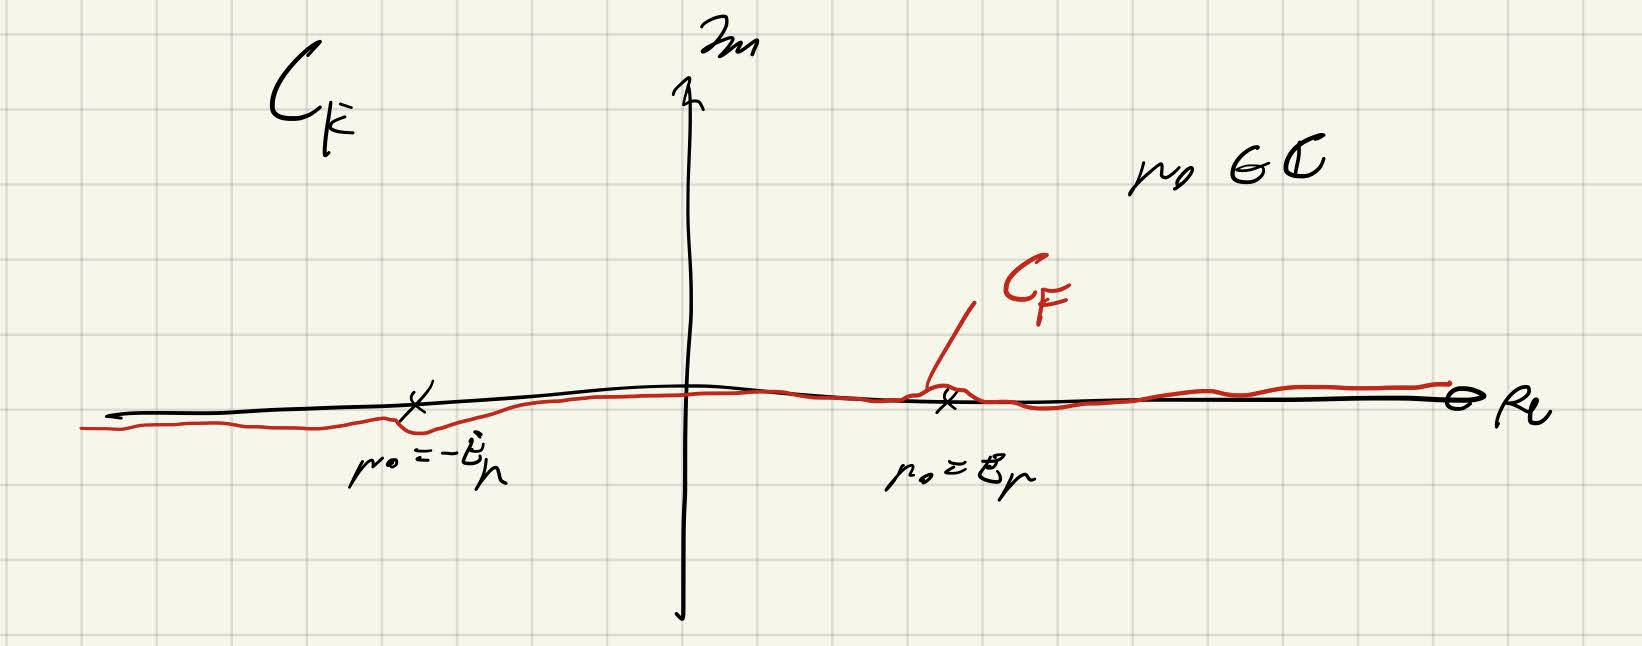
\includegraphics[width=7cm]{res/QFT/Feynman_contour}
\caption{Feynman Contour}
\label{feynman_contour}
\end{figure}

Now to prove our claim.

\begin{proof}
Notice that $|\mathcal{I}|$ depends only on $\text{Im}(p^0)$ meaning that if
$x^0 > y^0$ then we can complete the contour with a semicircle in the lower half
plane of the complex plane and apply Jordan's theorem since we are decaying
exponentially fast. In this case we only include the rightmost residue. On the
contrary if $x^0 < y^0$ we decay in the upper half plane and can complete with a
semicircle contour there to get the same result but now with the leftmost residue.
\end{proof}

Alternatively, one can justify this instead calculating

$$ \Delta_F(x - y) = \lim{\epsilon \to 0^+} \int \frac{d^4p}{(2\pi)^3} \frac{i
  e^{-ip_\mu (x - y)^\mu}}{p^2 - m^2 + i\epsilon} $$

\subsubsection{Wick's Theorem}

Now, this is fine for $T_2$ but what about arbitrary $l$? Here Wick's Theorem
comes into play. First let's define the \textbf{contraction} of $\phi_i, \phi_j$
to be (for example in the case $i=1, j=3$) as $\phi_1 \phi_2 \phi_3 \phi_4
\mapsto \Delta_F(x_1 - x_3) \phi_2 \phi_4$ where $\phi_i = \phi(x_i)$. Then we
define the symbol $\mathcal{C}(\phi_1 \dots \phi_n)$ to denote the sum over all
possible contractions (including all numbers of contractions - so no
contractions at all is a possibility, and so is 5 different contractions), then

\begin{theorem}
  \textbf{Wick's Theorem} states that
  $$ T(\phi_1 \dots \phi_n) = : \phi_1 \dots \phi_n : + \mathcal{C}(\phi_1 \dots
  \phi_n) $$
\end{theorem}

[End of lecture 13]

\begin{proof}
  We proceed by induction. If $n = 2$ then $T[\phi_1 \phi_2] = : \phi_1 \phi_2 :
  + \Delta_F(x_1 - x_2) = :\phi_1 \phi_2: + :(\phi_1 \phi_2): =
  :\mathcal{C}(\phi_1 \phi_2):$ (we use parentheses here in LateX to denote
  contraction). For the inductive step we write that if wlog $\forall i,  x_1
  \geq x_i$, then
\begin{align*}
T(\phi_1 \dots \phi_n) &= \phi_1 T(\phi_2 \dots \phi_n) \\
&= (\phi^+_1 + \phi^-_1) : \mathcal{C}(\phi_2 \dots \phi_n) \\
&= :\phi_1^- \mathcal{C}(\phi_2 \dots \phi_n): + :\phi_1^+ \mathcal{C}(\phi_2 \dots \phi_n): + : \sum_{i=2}^n [\phi_1^+, \phi_i] \mathcal{\phi_2 \dots \phi_{i - 1} \phi_{i + 1} \dots \phi_n} \\
&= :\phi_1 \mathcal{C}(\phi_2 \dots \phi_n): + \sum_{i = 2}^n :\mathcal{C}((\phi_1) \phi_i) \phi_2 \dots \phi_{i - 1} \phi_{i + 1} \dots \phi_n: \\
&= :\mathcal{C}(\phi_1 \dots \phi_n) 
\end{align*}
as required. Note here the we split the terms into a term where $\phi_1$ is
never contracted and a term where $\phi_1$ is always contracted (with every
$\phi_i$).
\end{proof}

Bizarrily, it turns out that the following quantity, the transition rate from
the vacuum to the vacuum, is nonzero, and this can be interpreted physically.
Anyways, here we find that

\begin{align*}
\bra{0} S \ket{0} &= \bra{0} Te^{\frac{1}{i} \frac{\lambda}{4!} \int d^4x \phi(x)} \ket{0} \\
&= \sum \frac{1}{l!} \left( \frac{1}{i} \frac{\lambda}{4!} \right)^l \int dx_1^4 \dots \int dx_l^4 M(x_1, \dots, x_l) \\
\end{align*}

For

$$ M(x_1, \dots, x_l) = \bra{0} T(\phi_1^4 \dots \phi_l^4) \ket{0} = \bra{0} :
\mathcal{C} (\phi_1^4 \dots \phi_l^4) \ket{0} $$

The only surviving terms are the terms where everything is contracted (or else
one of the vacuum states will be annihilated). The terms we then get can be
represented diagramatically (Feynman diagrams), such as 

$$ \bra{0} (\phi_1 \phi_1) (\phi_1 (\phi_1 \phi_2) (\phi_2 \phi_2) \phi_2)
\ket{0} $$

We can represent this by the following diagram:

\begin{figure}[H]
\centering
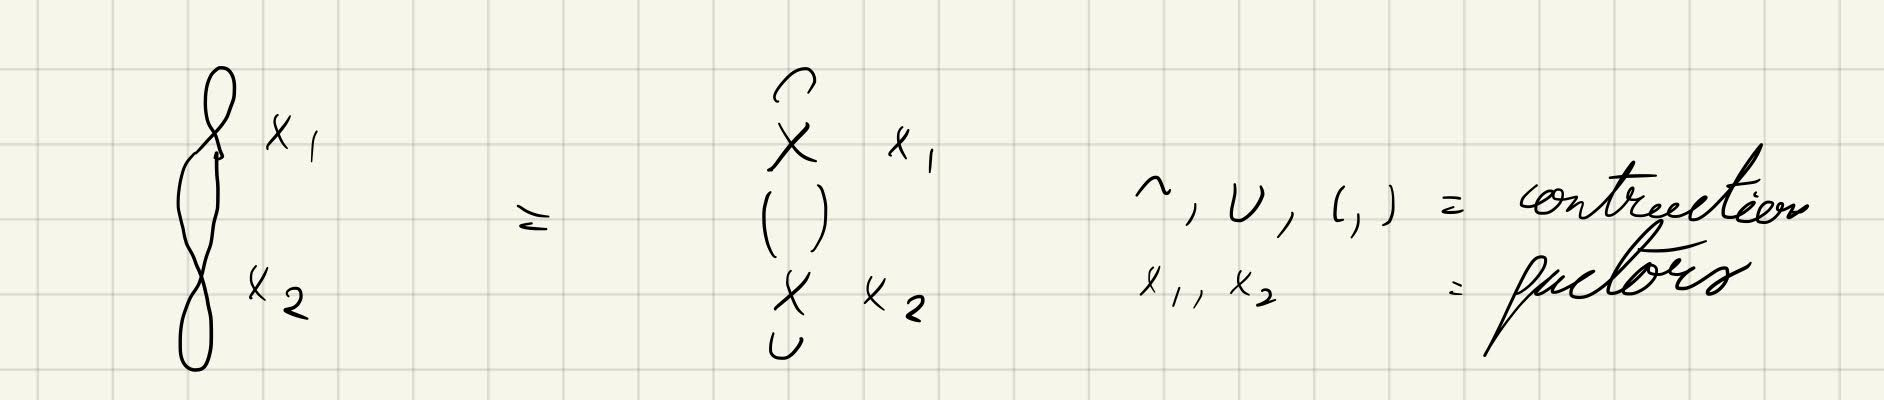
\includegraphics[width=10cm]{res/QFT/basic_feynman}
\caption{Simple Feynman Diagram}
\end{figure}

Here the number of vertices is $l$, and the number of connecting points at each
vertex is the number of times $\phi_i$ occurs. The contractions are then given
by the lines connecting the vertices.

\subsubsection{Scattering in Scalar-Yukawa}

We will work out one extended example of scattering in Scalar-Yukawa. Here we
have Lagrangian

$$ \mathcal{L} = \partial_\mu \psi^* \partial^\mu - M^2 \psi^* \psi +
\frac{1}{2} \partial_\mu \phi \partial^\mu \phi - \frac{M^2}{2} \phi^2 - g \phi
\psi^* \psi $$

We get ladder operators

\begin{align*}
  \phi(x) &= \int \frac{d^3p}{(2\pi)^3} \frac{1}{\sqrt{2 E_p}} (a_p e^{-ip \cdot x} + a^\dagger_p e^{ip \cdot x}) \\
  \psi(x) &= \int \frac{d^3p}{(2\pi)^3} \frac{1}{\sqrt{2 E_p}} (b_p e^{-ip \cdot x} + c^\dagger_p e^{ip \cdot x}) \\
  \psi^\dagger(x) &= \int \frac{d^3p}{(2\pi)^3} \frac{1}{\sqrt{2E_p}} (b^\dagger e^{ip \cdot x} + c_p e^{-i p \cdot x})
\end{align*}

We want to calculate the scattering amplitude between states

\begin{align*}
  \ket{i} &= \sqrt{2E_{p_1}} \sqrt{2E_{p_2}} b_{p_1}^+ b_{p_2}^+ \ket{0} \\
  \ket{f} &= \sqrt{2E_{p_1'}} \sqrt{2E_{p_2'}} b_{p_1'}^+ b_{p_2'}^+ \ket{0}
\end{align*}

Now to get a non-zero transition we need at least the terms $b^2, b^{\dagger
  2}$, which means we need to consider at least the second order term of the
Dyson equation, or in order words we use

$$ A_{i \to f} = \bra{f} S \ket{i} = T e^{\frac{g}{i} \int d^4 x \phi
  \psi^\dagger \psi} \approx A_{i \to f}^{(2)} = \frac{1}{2} \frac{g^2}{i^2}
\int d^4 x_1 \int d^4 x_2 M(x_1, x_2) $$

where

\begin{align*}
  M(x_1, x_2) &= \bra{f} T(\phi_1 \psi_1^\dagger \psi_1 \phi_2 \psi_2^\dagger \psi_2) \ket{i} \\
              &= \Delta_F^{(\phi)}(x_1 - x_2) \bra{f} : \psi_1^\dagger \psi_1 \psi_2^\dagger \psi_2 \ket{i} \\
              &= \Delta_F^{(\phi)} \bra{f} \psi_1^\dagger \psi_2^\dagger \psi_1 \psi_2 \ket{i} \\
              &= \Delta_F^{(\phi)} N
\end{align*}

since we care only for $b$ terms, so we can ignore $c$, and we've contracted
$\phi$ since nothing happens to those terms. [End of lecture 14] [The lecturer
mentions that his notes extend Wick's theorem to $\mathbb{C}$].

Writing

$$ N = \bra{f} \psi_1^\dagger \psi_2^\dagger \mathds{1} \psi_1 \psi_2 \ket{i} $$

where $\mathds{1} = \sum \ket{\psi} \bra{\psi}$  means we can write

$$ N = N_i N_f $$

where $N_i = \bra{0} \psi_1 \psi_2 \ket{f}$, and similar for $N_f$. Then

$$ N_i = \sqrt{2 E_{p_1}} \sqrt{2 E_{p_2}} \int \frac{d^3p}{(2\pi)^3} \int
\frac{d^3q}{(2\pi)^3} \frac{1}{\sqrt{2 E_p}} \frac{1}{\sqrt{2 E_q}} e^{-ip \cdot
  x_1 - i q \cdot x_2} \bra{0} b_p b_q b_{p_1}^\dagger b_{p_2}^\dagger \ket{0} $$

where we set $A = \bra{0} b_p b_q b_{p_1}^\dagger b_{p_2}^\dagger \ket{0}$ and
$[b_p, b_{p'}^\dagger] = (2\pi)^3 \delta(p - p')$ so

$$ A = (2\pi)^6 (\delta(p_1 - p) \delta(p_2 - q) + \delta(p_2 - p) \delta(p_1 -
q)) $$

(notice the apparent Bose symmetry). Consequently,

$$ N_i = e^{-i p_1' \cdot x_1 + i p_2' \cdot x_2} + e^{ip_2' \cdot x_1 + ip_1
  \cdot x_2 } $$

As such,

\begin{align*}
  A_{i \to f}^{(2)} &= \frac{1}{2} \frac{g^2}{i^2} \int d^4 x_1
                      \int d^4 x_2 N_f N_i
                      \int \frac{d^4k}{(2\pi)^4}
                      \frac{i e^{ik(x_1 - x_2)}}{k^2 + m^2 + i \epsilon} \\
                    &= \frac{g^2}{2i^2} \int \frac{d^4k}{(2\pi)^4}
                      \frac{i}{k^2 - m^2 + i\epsilon} \int d^4 x_1 \int d^4 x_2
                      \left( e^{ix_1 \cdot (k - p'_1 -p_1)} e^{ix_2 \cdot (k - p_2' + p_2)}
                      + e^{i x_1 \cdot (k + p_2' - p_1) e^{ix_2 \cdot (k - p_1' + p_2)}} \right)
\end{align*}

where the two terms are related by swapping $x_1, x_2$. Doing the $x_1, x_2$
integral using $\int d^4x e^{ipx} = (2\pi)^4 \delta(p)$ we get

$$ A_{i \to f}^{(2)} = i(-ig)^2 (2\pi)^4 \delta(p_1 + p_2 - p_1' - p_2') \left(
  \frac{1}{(p_1 - p_1')^2 - m^2 + i\epsilon} + \frac{1}{(p_1 - p_1')^2 - m^2 +
    i\epsilon} \right) $$

Now, $(p_1 - p_1')^2, (p_2 - p_2')^2 < 0$ means that we can just set $\epsilon =
0$.

\subsubsection{Feynman Diagrams}

We can systemise the previous calculations through the use of Feynman diagrams.
In particular, we see that terms of $\bra{f} S - 1 \ket{i}$ correspond to
Feynman diagrams.

In Feynman diagrams, we represent terms via lines (or \textbf{propagators}) and
connect these according to the Hamiltonian. We also always specify a direction
for time. So if time flows from left to right we get

\begin{figure}[H]
  \centering
  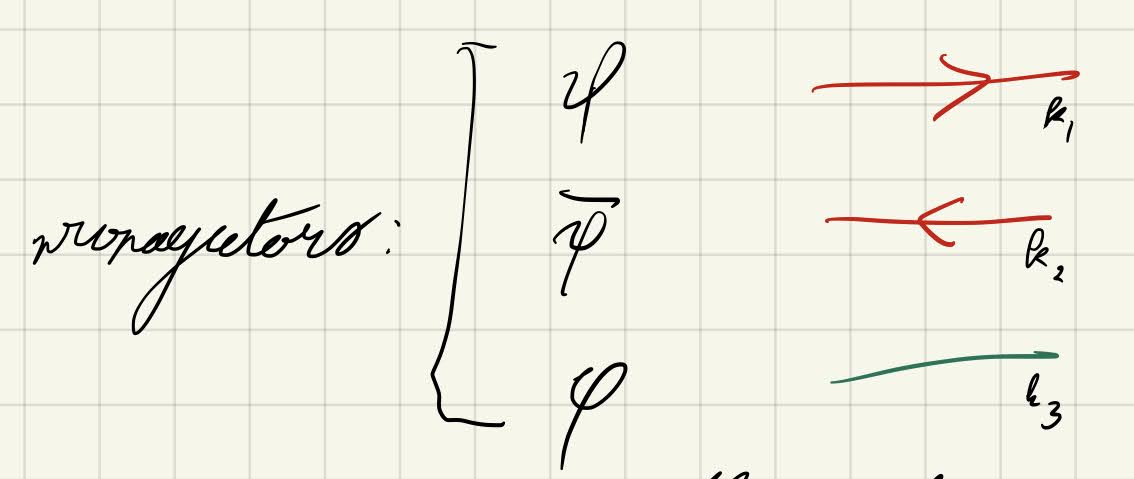
\includegraphics[width=5cm]{res/QFT/feynman_propagators}
  \caption{Feynman Diagram Propagators}
  \label{feynman_propagators}
\end{figure}

meaning that in our previous example we get leading terms as

\begin{figure}[H]
  \centering
  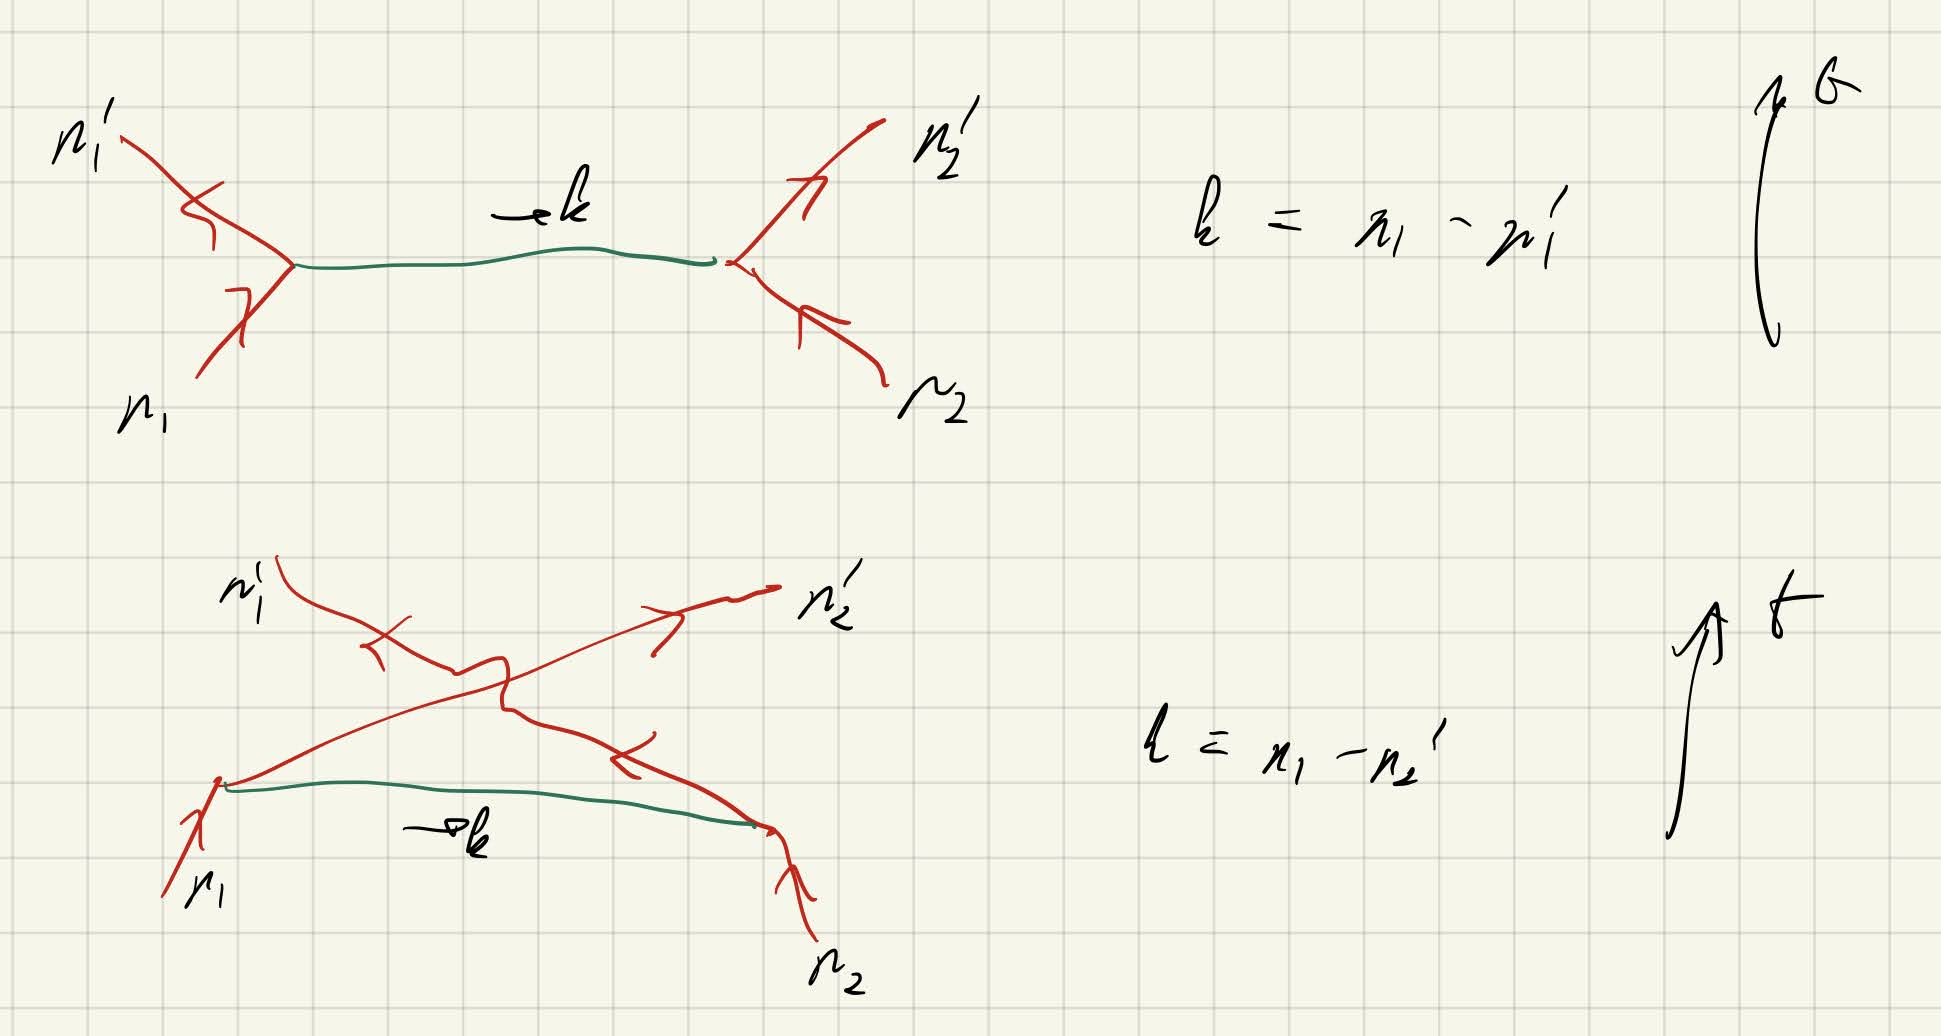
\includegraphics[width=9cm]{res/QFT/feynman_example}
  \caption{Feynman Diagram Leading Terms}
  \label{feynman_example}
\end{figure}

Note that here every propagator has a momentum associated with it, and that
particles/anti-particles have ``directions'' associated with them. Now to
convert these to calculations we have the following correspondance:

\begin{figure}[H]
  \centering
  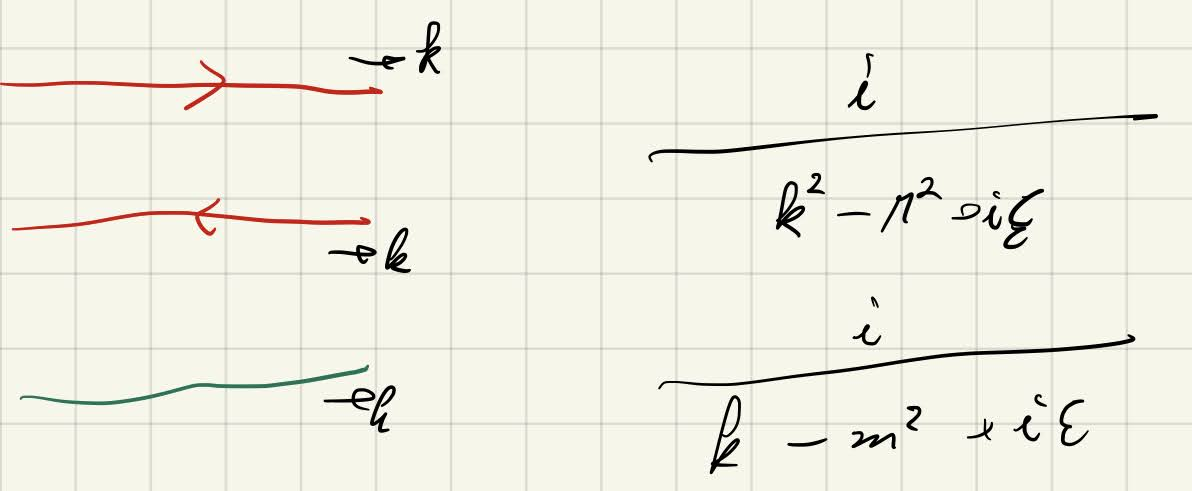
\includegraphics[width=5cm]{res/QFT/feynman_correspondance}
  \caption{Feynman Propagator Meaning}
  \label{feynman_correspondance}
\end{figure}

\begin{figure}[H]
  \centering
  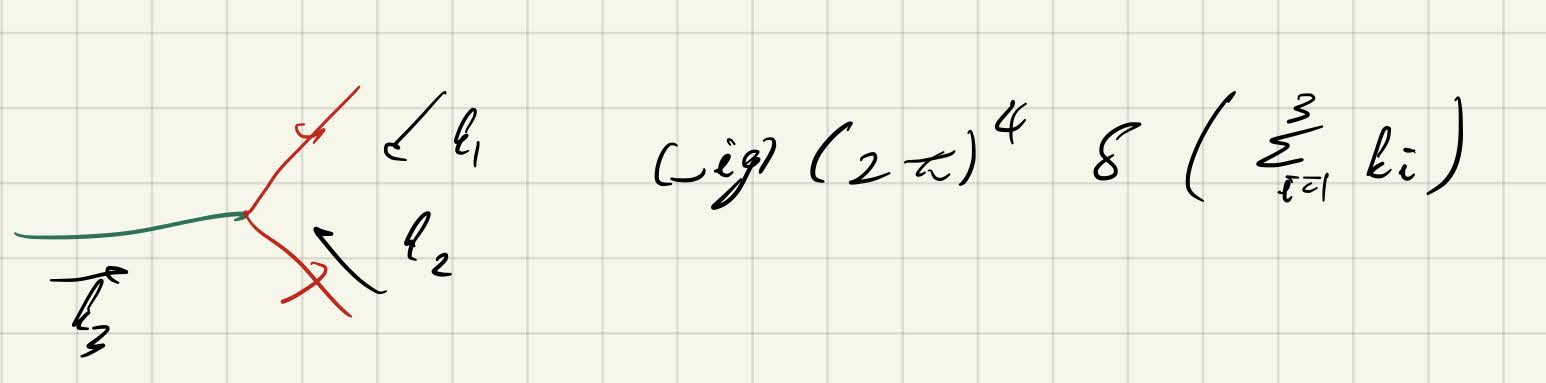
\includegraphics[width=7cm]{res/QFT/feynman_correspondance_2}
  \caption{Feynman Vertex Meaning}
  \label{feynman_correspondance_2}
\end{figure}

Consequently, the top diagram we had correspondance to (to appropritae order)

$$ A_{i \to f} |_{O(g^2)} = i(-ig)^2 \left( \frac{1}{(p_1 - p_1')^2 - m^2} +
  \frac{1}{(p_2 - p_2') - m^2} \right) (2\pi)^4 \delta(p_1 + p_2 - p_1' -
p_2') $$

That completes the Feynman rules for this theory!

\section{Fermions}

We've now completed the scalar field theory of the course, and now want to move
to scalar fields of spins $1/2, 1$. To do so, we now need to start considering
representation theory. Now, what is ``spin'' here, just so we see how we might
generalise. We can roughly define spin to be the angular momentum of a
particular in its rest frame, $\bra{0} J \ket{0}$. Non-relativistically, we get
$2s + 1$ such spin states.

\subsection{Relativistic Spin}

To represent relativistic spins, it turns out we have to use representations of
the Lorentz group. [End of lecture 15] For that, let's review how representation
theory fits into quantum field theory. In particular, we move from a scalar
field to a vector field, and we specify how it transforms via a representation
$D$ of the Lorentz group such that

$$ \psi_A (x) \mapsto \psi_A'(x') = D(\Lambda)_{AB} \psi_B(\Lambda^{-1} x) $$

How can we get more representations? In general, we have a Lie group $G$, which
is quite hard to describe, being on a manifold. Fortunately, we can greatly
simplify our analysis by focusing on the Lie algebra $\mathbb{L}(G)$, which is
linear approximation of the Lie group near the identity. We then can use the
exponential map $\text{Exp} : \mathbb{L}(G) \to G$ to map back into the Lie
group. This, however, is just a local bijection, but for most purposes this is
enough. A representation of a Lie algebra is a map $R : \mathbb{L}(G) \to
\text{Mat}_N (\mathbb{C})$ that is linear and preserves the Lie bracket

$$ R([X, Y]) = [R(X), R(Y)]. $$

where we can then recover the Lie group by using $D(\Lambda) = Exp(R(X))$.
However, this is not a surjective map, and only gives us one representation of a
large set of possible representations. More importantly, we dont actually get a
representation itself, but rather of the cover of $G$, denoted $\tilde{G}$, just
like us getting $SL(2, \mathcal{C})$ as a double-cover of $SO(3, 1)$. This is
important to know since we will actually be using representations of the cover,
not the group itself.

As such we see that for proper Lorentz transformations $\Lambda = e^\omega$ we
have $\omega$ antisymmetric (by considering on a linear level $\Lambda \eta
\Lambda^T = \eta$). Consequently the Lie alegbra of the Lorentz transformations
is just the set of antisymmetric $4\times 4$ real matrices.

Antisymmetry means that treated as a linear space, this space has dimension
$\frac{1}{2} 4 \cdot 3 = 6$ (3 rotations and 3 boosts) which can express with
the basis $M^{\rho \sigma} = (M^{\rho \omega})^{\mu \nu} = \eta^{\rho \mu}
\eta^{\sigma \nu} - \eta^{\sigma \mu} \eta^{\rho \nu}$ where the generators are
labelled such that $M^{\rho \sigma} = -M^{\sigma \rho}$. We can then write a
general element of the Lie algebra $\mathbb{L}(G_L)$ is

$$ \omega^\mu_{\ \nu} = \frac{1}{2} \Omega_{\rho \sigma} (M^{\rho
  \sigma})^\mu_{\ \nu} $$

where the parameters $\Omega_{\rho \sigma} = -\Omega_{\rho \sigma}$ (the
symmetric part does not contribute). To finish showing that this truly is a
representation of the Lie Algebra we can observe that

$$ [M^{\rho \sigma}, M^{\tau \nu}] = \eta^{\sigma \tau} M^{\rho \nu} -
\eta^{\rho \tau} M^{\sigma \nu} + \eta^{\rho \nu} M^{\sigma \tau} - \eta^{\sigma
\nu} M^{\rho \tau} $$

[why?] A trick due to Dirac in organising representations of the Lorentz group is to
start with the Clifford alegbra $\gamma^\mu$ for $\mu = 0, 1,2 3$ with the
property

$$ \{ \gamma^\mu, \gamma^\nu \} = 2 \eta^{\mu \nu} I $$

This is satisfied by the Pauli matrices, however, there are only 3 of those, and
it turns out the lowest-dimensional set of 4 matrices satisfying these
properties are

\begin{align*}
\gamma^0 &= 
\begin{pmatrix}
& I \\
I & 
\end{pmatrix} \\
\gamma^i &=
\begin{pmatrix}
& \sigma^i \\
-\sigma^i & 
\end{pmatrix}
\end{align*}

The Lorentz Lie Algebra generators then arise (for reasons not discussed here)
as

$$ S^{\rho \sigma} = \frac{1}{4} [\gamma^\rho, \gamma^\sigma] = \frac{1}{2}
\gamma^\rho \gamma^\sigma - \frac{1}{2} \eta^{\rho \sigma} $$

On example sheet 3, one shows that as required

$$ [S^{\mu \nu}, S^{\rho \sigma}] = \eta^{\nu \rho} S^{\mu \sigma} - \eta^{\mu
  \rho} S^{\nu \sigma} + \eta^{\mu \sigma} S^{\nu \rho} - \eta^{\nu \sigma}
S^{\mu \rho} $$

We can then exponentiate to get a representation of the double cover $SL(2,
\mathbb{C})$.

$$ \Lambda = \text{Exp}(\frac{1}{2} \Omega_{\rho \sigma} M^{\rho \sigma}),
S(\Lambda) = \text{Exp}(\frac{1}{2} \Omega_{\rho \sigma} S^{\rho \sigma}) $$

(we establish a representation of the Lorentz group by establish a simple
correspondance between generators of the Lorentz group as a vector space and
similar generators for the representation). ($M$s generate the Lie algebra, $S$s
generate the Lie group) [End of lecture 16]

Now, for rotations we can write

$$ \Omega_{ik} = -\epsilon_{ijk} a^k $$

and so the Spinor representation is given by (for $i \neq j$)

$$ S^{ij} = \frac{1}{4} [\gamma^i, \gamma^j] = \frac{1}{2} \gamma^i \gamma^j =
-i \frac{1}{2} \epsilon^{ijk}
\begin{pmatrix}
  \sigma^k & \\
  & \sigma^k
\end{pmatrix}
$$

in the Chiral representation. This corresponds to Lorentz transformation

$$ S(\Lambda) = \text{Exp} (\frac{1}{2} \Omega_{ij} S^{ij}) =
\begin{pmatrix}
  e^{ia \cdot \sigma / 2} & \\
  & e^{ia \cdot \sigma / 2}
\end{pmatrix}
$$

Consequently for a rotation around the $z$-axis where $a^1 = a^2 = 0$ we get

$$ S(a^3) = S(\Lambda) =
\begin{pmatrix}
  e^{i a^3 / 2} & & & \\
  & e^{-ia^3 / 2} & & \\
  & & e^{i a^3 / 2} & \\
  & & & e^{-ia^3 / 2}
\end{pmatrix} $$

for $\Lambda = \text{Exp}(\frac{1}{2} \Omega_{ij} M^{ij})$. In this case we see
that

$$ \Lambda(a^3) = \text{Exp}(-a^3 M^{12}) $$

and

$$ M^{12} =
\begin{pmatrix}
  0 & & & \\
  & 0 & -1 & \\
  & 1 & 0 & \\
  & & & 0
\end{pmatrix} $$

meaning that by pairing sines and cosines

$$ \Lambda(a^3) =
\begin{pmatrix}
  0 && \\
  & M(a^3) & \\
  && 0
\end{pmatrix} $$

for standard rotation matrix

$$ M(a^3) =
\begin{pmatrix}
  \cos(a^3) & \sin(a^3) \\
  -\sin(a^3) & \cos(a^3)
\end{pmatrix} $$

Note here that for $a^3 = 2\pi$ we get $\Lambda(a^3) = I$. However, the spinors
in this case correspond to

$$ S(a^3 = 2\pi) = - I $$

confirming indeed that we have a representation of the double-cover and not the
space itself. This in particular, is a characteristic of fermion
representations. 

\subsection{Spinor Representations}

Our Clifford algebra forms a ``invariant tensor'' in the sense that [what
exactly is meant here]

$$ S^{-1} (\Lambda) \gamma^\mu S(\Lambda) = \Lambda^\mu_{\ \nu} \gamma^\nu $$

We only verify this infinitesimally where we see that to first order

\begin{align*}
  \Lambda &= \text{Exp} \left( \frac{1}{2} \Omega_{\rho \sigma}
            M^{\rho \sigma} \right) \\
          &\approx \left( S^\mu_{\ \nu} + \frac{1}{2} \Omega_{\rho \sigma}
            (M^{\rho \sigma})^\mu_{\ \nu}) \right)
            \gamma^\nu + O(\Omega^2) \\
          &= \gamma^\nu + \frac{1}{2} \Omega_{\rho \sigma}
            (M^{\rho \sigma})^\mu_{\ \nu} \gamma^\nu + O(\Sigma) \\
          &= \gamma^\mu + \frac{1}{2} \Omega_{\rho \sigma} (\eta^{\rho \mu} \gamma^\sigma
            - \eta^{\sigma \mu} \gamma^\rho)
\end{align*}

And so on the LHS we find

\begin{align*}
  S(\Lambda) &= \text{Exp} \left( \frac{1}{2} \Omega_{\rho \sigma}
               S^{\rho \sigma} \right) \\
             &\approx I - \frac{1}{2} \Sigma_{\rho \sigma} S^{\rho \sigma}
               \cdot \gamma^\mu \cdot \left( I + \frac{1}{2} \Omega_{\rho \sigma}
               S^{\rho \sigma} \right) + O(\Sigma^2) \\
             &\approx \gamma^\mu + \frac{1}{2} \Omega_{\rho \sigma}
               [\gamma^\mu, S^{\rho \sigma}] + O(\Omega^2)
\end{align*}

As such we get equality to linear order, or in other words, we get

$$ [\gamma^\mu, S^{\rho \sigma}] = \eta^{\rho \sigma} \gamma^\sigma -
\eta^{\sigma \mu} \gamma^\rho $$

\subsection{Spinor Fields}

So how do we construct fields (and eventually equations of motion) in this case.
For field $\psi : \mathbb{R}^{3, 1} \to \mathbb{C}^4$ we have transformation
property

$$ \psi^\alpha(x) \to \psi'^\alpha(x') = S(\Lambda)^\alpha_\beta
\psi^\beta(\Lambda^{-1} \cdot x) = S(\Lambda) \cdot \psi(\Lambda^{-1} x) $$

which fortunately satisfies the key property that under a $2\pi$ rotation we
have $\psi \mapsto -\psi$. This is all nice and well, but we need a Lorentz
transformation that is Lorentz invariant, and it is not immediately obvious how
we construct that from these terms that transform in a more complex manner.
First we observe that

$$ \partial_\mu \psi(x) \mapsto (\Lambda^{-1})^\nu_{\ \mu} S(\Lambda) \cdot
\partial_\nu (\Lambda^{-1} \cdot x) $$

and 

$$ \psi^\dagger_\alpha(x) \mapsto \psi^\dagger \cdot S(\Lambda)^\dagger $$

Unlike before $S(\Lambda)$ is not always unitary, which means $\psi^\dagger
\cdot \psi$ is no longer a scalar quanttiy. Furthermore, we have the theorem
that

\begin{theorem}
A simple non-compact Lie group has no non-trivial finite dimensional unitary
representation.
\end{theorem}

which severely restricts our options here. As such, notice first that for our
Clifford algebra using the Chiral representation we get

$$ \{\gamma^\mu, \gamma^\nu\} = 2\eta^{\mu \nu} I, (\gamma^0)^2 = I,
(\gamma^i)^2 = -I, (\gamma^i)^\dagger = -\gamma^i, (\gamma^0)^\dagger =
\gamma^0 $$

Consequently we can see that

$$ (\gamma^\mu)^\dagger = \gamma^0 \gamma^\mu \gamma^0 $$

[End of lecture 17]

\end{document}